\documentclass[english]{article}



\usepackage{graphicx}
\usepackage[hidelinks]{hyperref}
\usepackage{grffile}
\usepackage[T1]{fontenc}
\usepackage{babel}
\usepackage{float}
\usepackage{tabu}
\usepackage{ragged2e}
\usepackage{textcomp}
\usepackage{amstext}
\usepackage[final]{pdfpages}
\usepackage{caption}
\usepackage{color}


\graphicspath{{../Pictures/}}


\begin{document}
	
	
	\begin{figure}[H]
		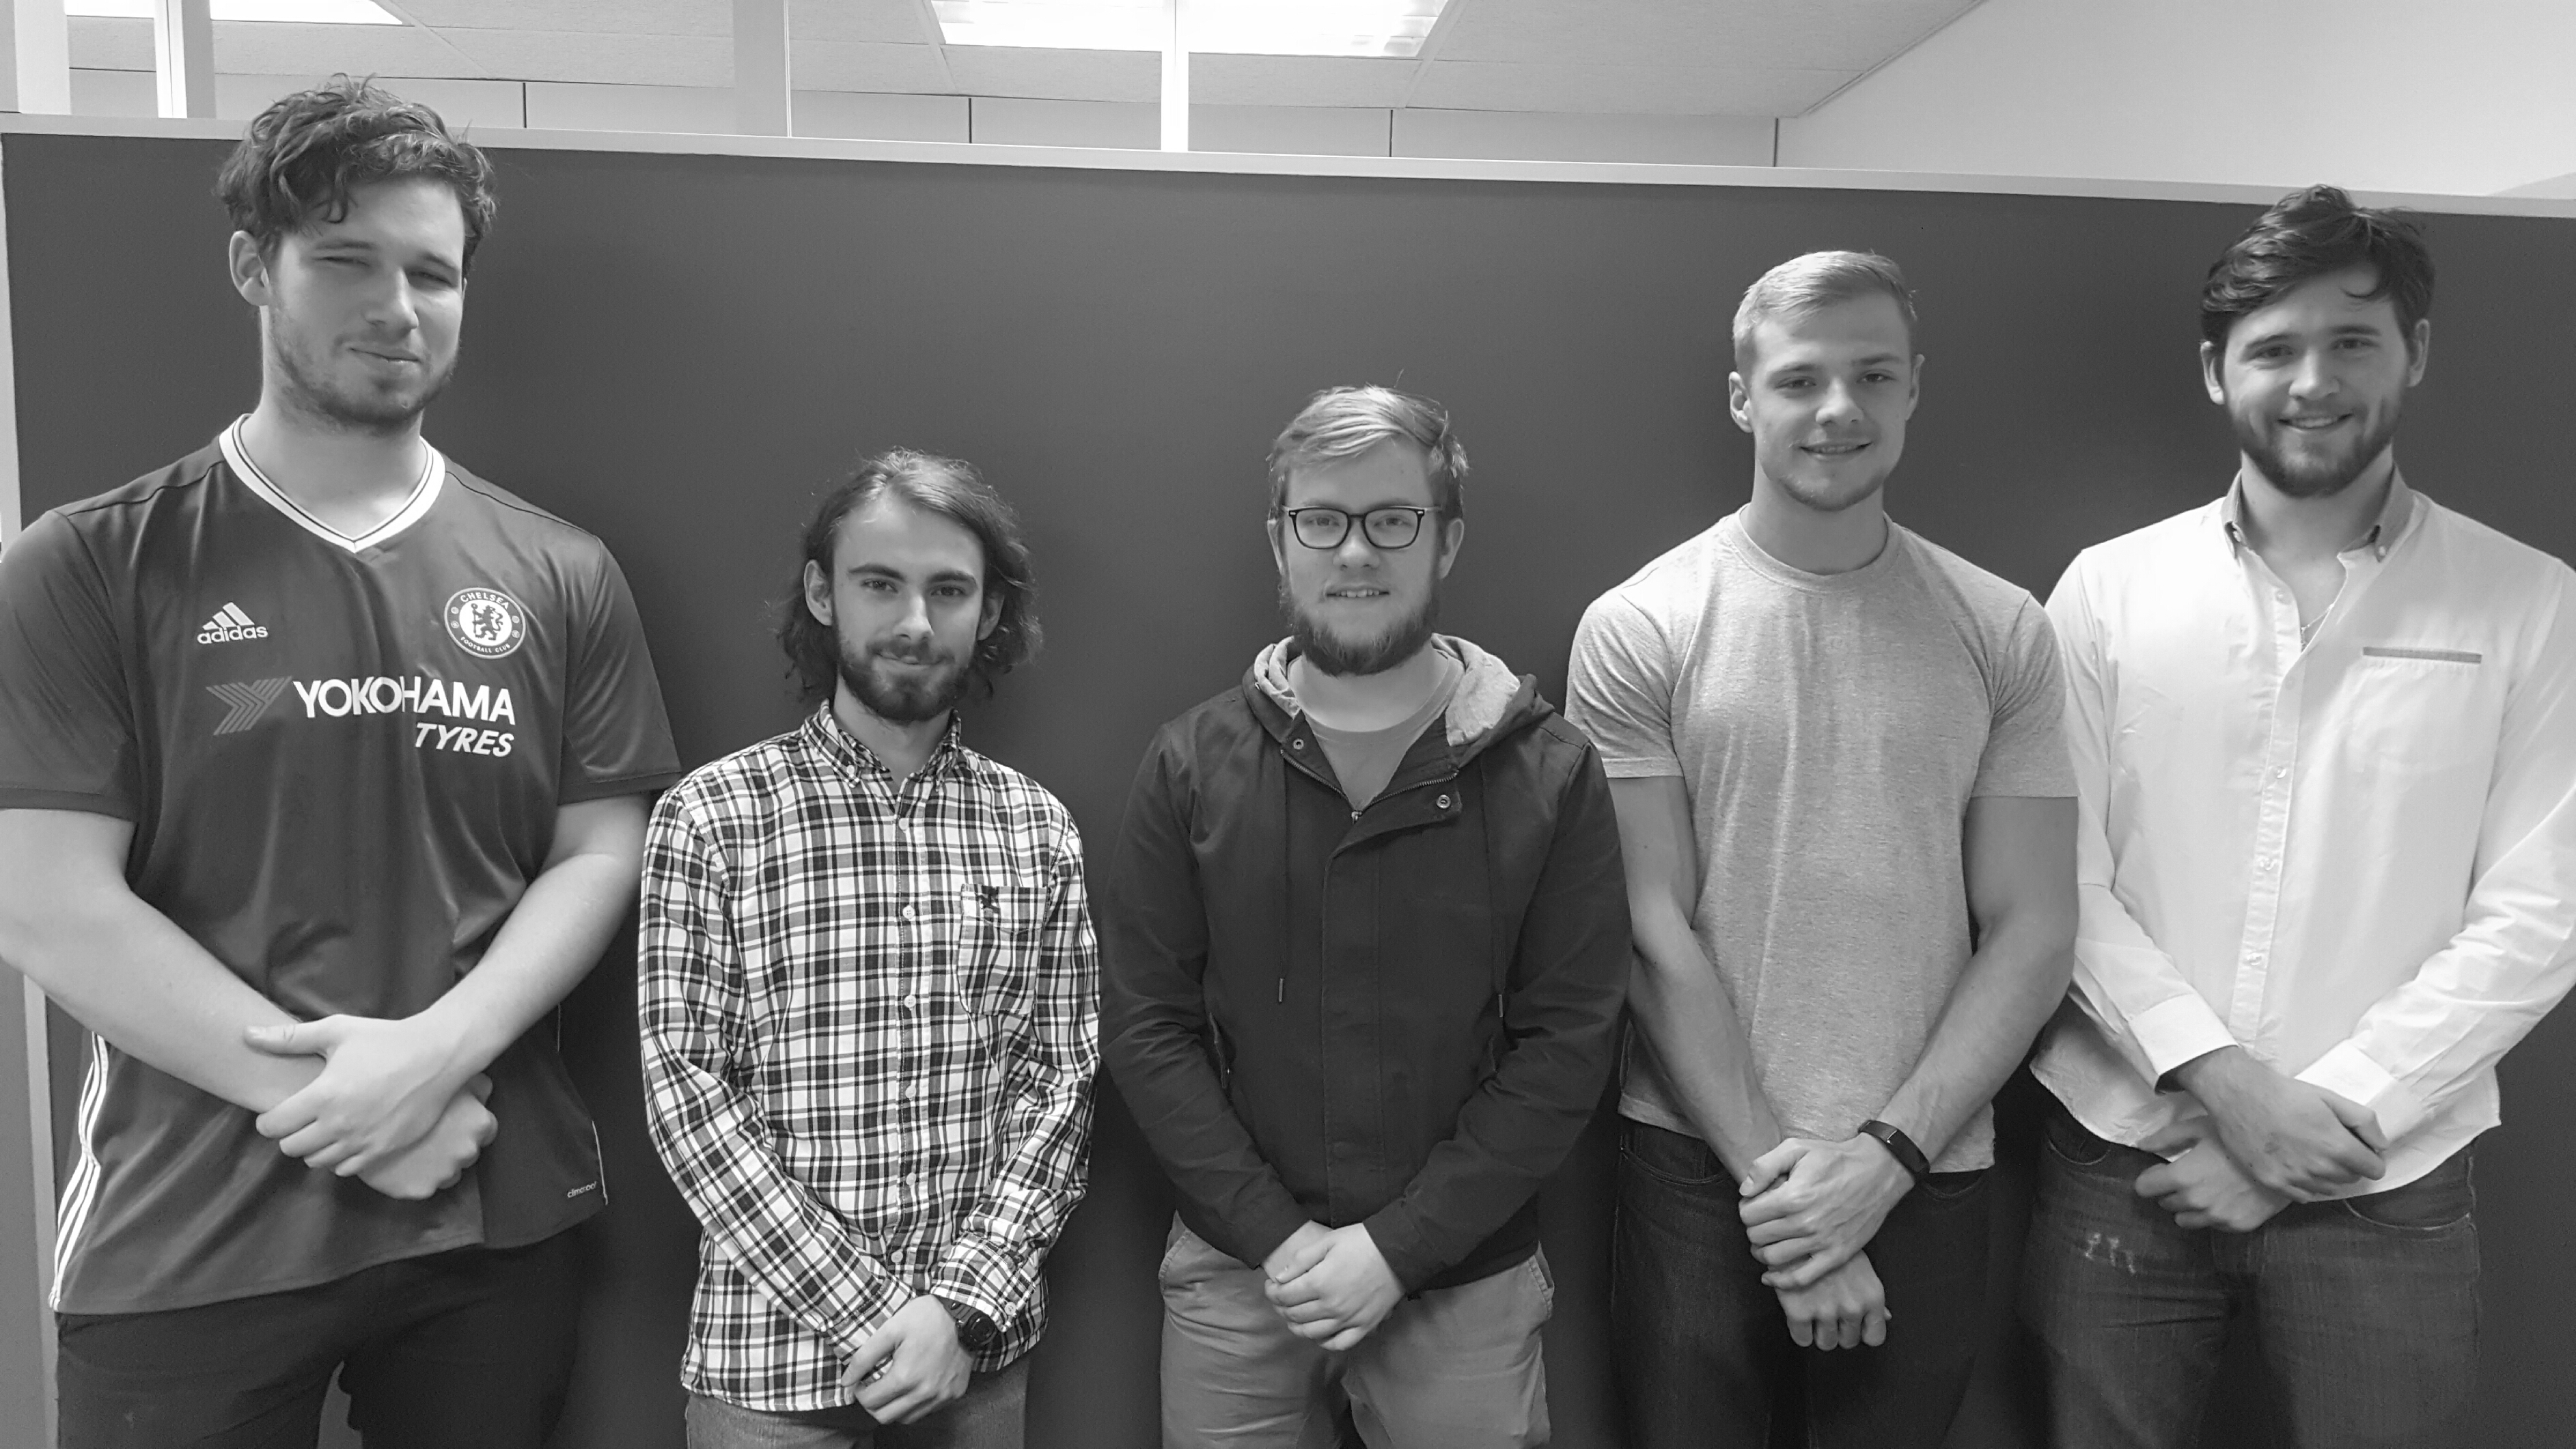
\includegraphics[width=\linewidth]{Team/teamphoto.jpg}
	\end{figure}

	\begin{figure}[H]
		
\includegraphics[width=\linewidth]{Team/teamtitle.jpg}
	\end{figure}

	\begin{figure}[H]
		
\includegraphics[width=\linewidth]{documenttitle.jpg}
	\end{figure}

	\begin{figure}[H]
		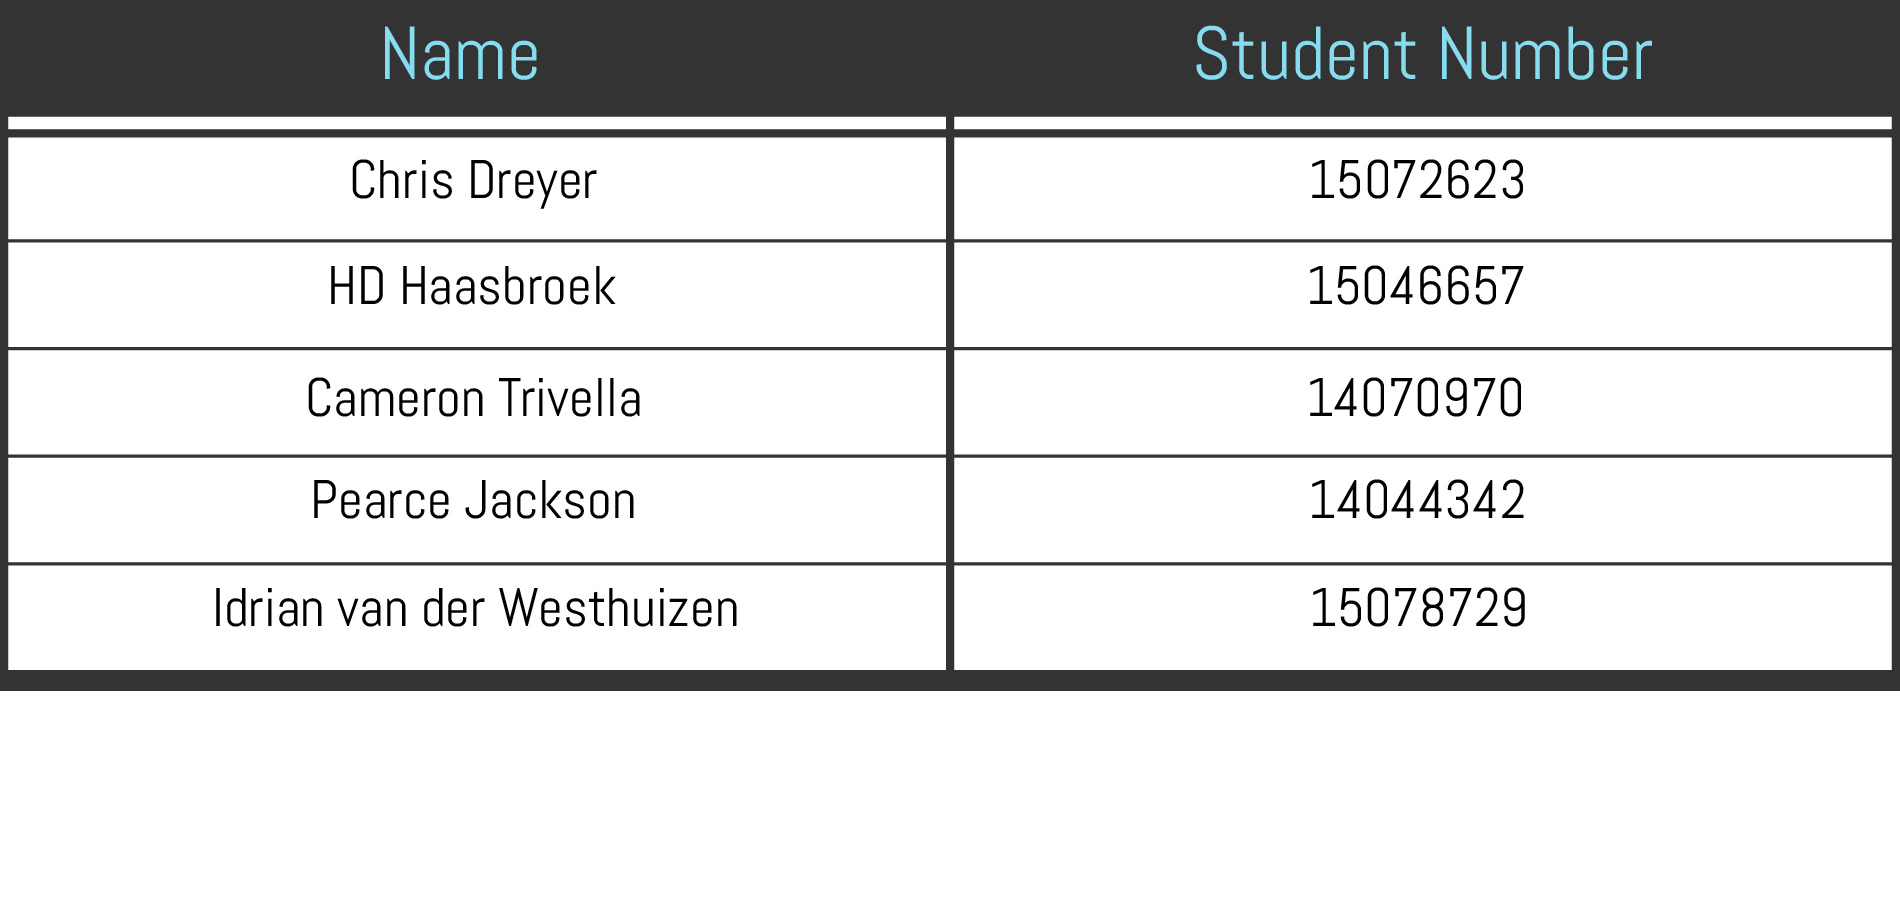
\includegraphics[width=\linewidth]{Team/teamtable.jpg}
	\end{figure}
	
	\pagenumbering{gobble}
	\newpage
	\tableofcontents
	
	\pagenumbering{arabic}
	\newpage

	\section{Introduction}
	
		\subsection{Purpose}
		
		This SRS document aims to stipulate the requirements of the voxc.js library to aid in the development process and to ensure that a functional and usable product is delivered.
		
		\subsection{Product Scope}
		
		Voxc.js is meant to be an easy to use and easy to maintain JavaScript library, similar to how three.js is a library for WebGL. The purpose of the project is to provide users a way to import Voxel models into a webpage that would be using the Voxc.js library and use these Voxel models as a coordinate system to create newly genereated mesh object according to a rules file with a specified structure. The user will then be able to export the textured and rendered object.
		
		\subsection{References}
		
		\color{blue}
		\url{http://www.oskarstalberg.com/game/house/Index.html}
		\newline
		\\\url{https://voxel.codeplex.com/}
		\newline
		\\\url{https://pages.github.com/}
		\newline
		\\\url{http://threejs.org/}
		\newline
		\\\url{http://coffeescript.org/}
		\newline
		\\\url{http://es6-features.org/#Constants}
		\newline
		\\\url{http://www.typescriptlang.org/}
		\newline
		\\\url{http://www.codebelt.com/typescript/typescript-es6-modules-boilerplate/}
		\newline
		\\\url{http://giacomotag.io/typescript-webpack/}
		\color{black}
		
	\pagebreak
	
	\section{External Interface Requirements}
	
		\subsection{User Interfaces}
		The users should be able to interface with voxc.js through our web interface that will be hosted on Github Pages. They will mainly be using a laptop or a desktop to interface with the library. However the library itself should be able to interface with any website on any device with a web browser that has support for WebGL.
		\\\\
		The end users should thus be able to use the library for any webinterface they program that allows for the use of WebGL.
		
		\subsection{Software Interfaces}
		The system should incorporate several different languages in order to function. For the rules file, JSON objects should be 
		used so that the users can manipulate the file in any text editor based on set conventions and structure. 
		\\\\
		MagicVoxel should be used for the creation and manipulation of voxel objects. The library should be able to handle the .obj filetype for the voxel objects.
		\\\\
	 	The library should use TypeScript as the JavaScript variant to enable future developers and current developers to debug easier. The library should run on all major internet browsers that support WebGL.
	 	\\\\
	 	The library should be compiled together using webpack, as to allow end users to simply download a single Javascript file for use in their own projects.
		
		\subsection{Communications Interfaces}
		HTTP will be used to handle GET and POST requests and FTP will be used for file uploads and downloads.
		\\\\
		Due to the way Chrome handles the loading of local files it should be made clear to the user that in order to run anything locally that they would need to make use of some sort of server such as a node server or even xampp.
	\pagebreak
	
	
	\section{System Requirements}
	\begin{tabular}{||c | c||} 
		\hline
		Requirement ID & Requirement description \\ [0.5ex] 
		\hline\hline
		R1 & User should be able to upload their files from the webinterface \\ 
		\hline
		R1.1 & User uploads valid .obj, png and rule file \\ 
		\hline
		R1.2 & User uploads valid .obj and rule file. Should default png \\
		\hline
		R1.3 & User uploads valid .obj and png. Should default rule file \\
		\hline
		R1.4 & User uploads valid .obj. Should default png and rule file \\
		\hline
		R1.5 & User uploads valid js arrays \\
		\hline
		R1.6 & User uploads valid 3D matrix \\
		\hline
		R1.7 & User uploads valid array of images \\
		\hline
		R2 & Should be able to convert .obj to JSONMAtrix \\ 
		\hline
		R3 & Should be able to convert array of images to JSONMAtrix \\ 
		\hline
		R4 & Should be able to convert JSONMAtrix to Three-js mesh \\ 
		\hline
		R4.1 & Should be able to create visual 3D-matrix \\ 
		\hline
		R4.2 & Should be able to apply rule file \\ 
		\hline
		R4.2.1 & Should apply textures and change matrix according to rule file \\ 
		\hline
		R4.2.2 & Should be able to apply rule file with use of cellular-automata\\ 
		\hline
		R5 & Should be able to convert Three-js mesh into .obj\\ 
		\hline
		R5.1 & Converted .obj should be exportable/downloadable\\ 
		\hline
		R5.2 & Should contain all textures for ease of use\\ 
		\hline	
	\end{tabular}
	
		\pagebreak
	\section{System Features}		
		\subsection{File upload}

			 \subsubsection{Description and Priority}
			 	This feature will be needed for the webinterface, but is not required, thus it has a low priority. The feature will get user input in the form of a file upload, the feature should be able to determine what file is being uploaded and then through use of a strategy method determine the most valid course of action, i.e. selection of the 1st converter.
			 	
			 	\subsection{OBJ file upload with rules file}
			 	\begin{figure}[h]
			 		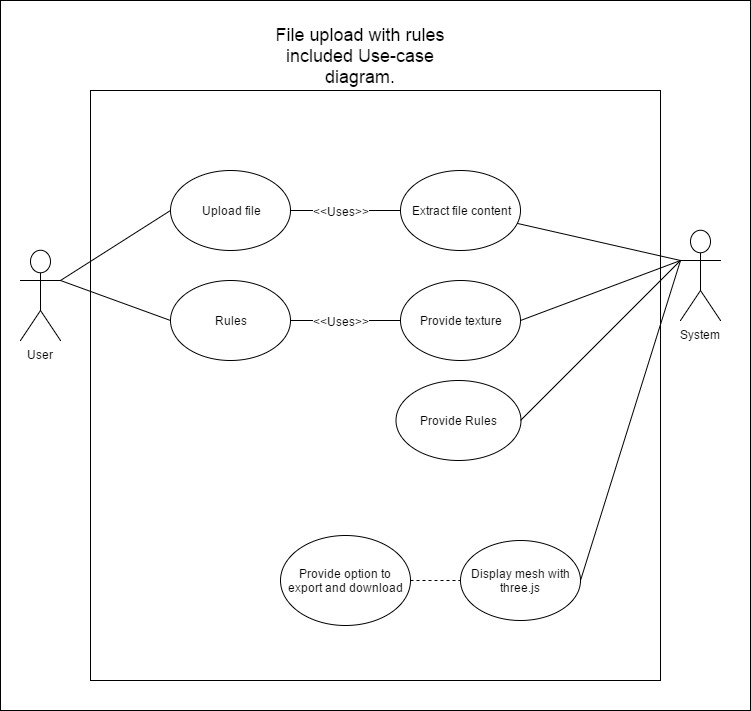
\includegraphics[width=\textwidth]{Use Cases/rules.jpg}
			 		\caption{Use Case Diagram for User upload with rules }
			 	\end{figure}
			 \subsubsection{Stimulus/Response Sequences}
			 	Stimulus: The user uploads his file with the rules file included.\\
			 	Response sequences: The system responds by using the files the user uploaded to extract them.\\\\
			 	 The system then determines the appropriate 1st converter and also provides the later converters with the uploaded rule file.
			 	 
			 \subsection{File upload without rules feature}
				\begin{figure}[h]
					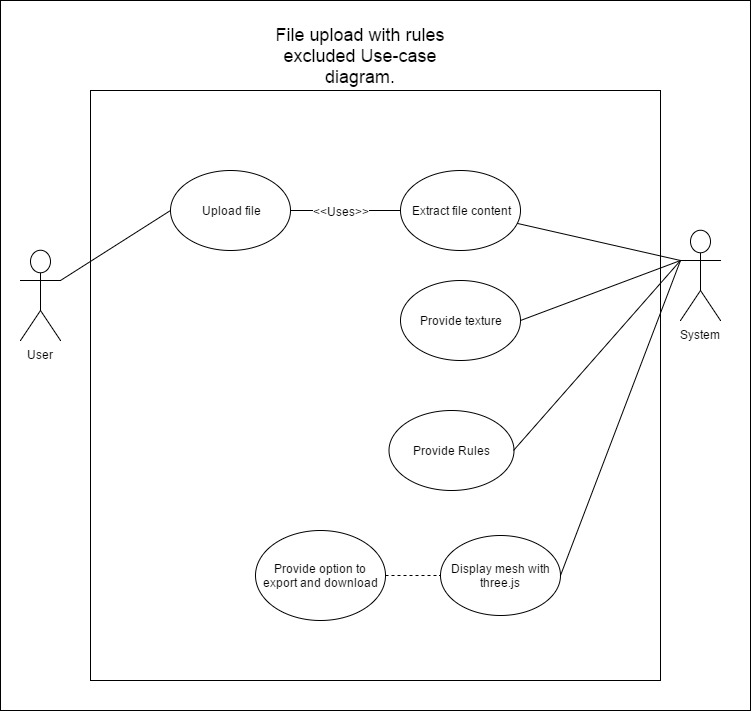
\includegraphics[width=\textwidth]{Use Cases/norules.jpg}
					\caption{Use Case Diagram for User upload with rules }
				\end{figure}
			 \subsubsection{Stimulus/Response Sequences}
			 	Stimulus: The user uploads his file with the rules file excluded.\\
			 	Response sequences: The system responds by using the files the user uploaded to extract them.\\\\
			 	 The system then determines the appropriate 1st converter and also provides the later converters with the default rule file provided by the system. 
	\pagebreak
	
		\subsection{ObjToArray}
		\subsubsection{Description and Priority}
			This feature is the first step in the .obj file upload process and is required in order to allow the use of subsequent converters. It is thus of medium-high priority as the user need not upload or use an obj file, but can instead use one of the other initial converters for different file types.\\\\
			The ObjToArray class should take in and obj file, preferably one created with the use Magicavoxel, that would then convert it into a JSONMatrix array containing the color values of each voxel from the obj.
			
	\pagebreak
		\subsection{ArrayToMesh}
		\subsubsection{Description and Priority}
		This feature is an intermediate/bridging converter where the outputs of each initial converter would need to go through in order to apply the rule file and create the new 3D object a.k.a the new mesh. It is beacuse all converters need to go through this converter eventually that it has a very high priotity, because if this converter fails then all other before and after converters would fail as a result.\\\\
		The converter will start using the outputted JSONMatrix of previous converters as a coordinate system in order to determine where textures and objects should go according to the supplied rule file. 
		
	\pagebreak
	\subsection{MeshToObj}
	\subsubsection{Description and Priority}
	This feature provides one of the end products of the converter pipeline and is optional to the end user, but is asked for by the client. It thus has a medium priority as most end users would probably ignore this feature, but because the client wants to use it, its priority is elevated.
	
	\pagebreak
	\subsection{IMGsToArray}
	\subsubsection{Description and Priority}
	This feature is the first step in the array of images file upload process and is required in order to allow the use of subsequent converters. It is thus of medium-high priority as the user need not upload or use an image array file, but can instead use one of the other initial converters for different file types.\\\\
	The IMGsToArray class should take in and array of images that would then be converted into a JSONMatrix array containing the color values of each pixel from the array of images.
	
	\pagebreak
	
	\section{Other Nonfunctional Requirements}
	
		\subsection{Performance Requirements}
		\subsubsection {Time to respond to an uploaded file}
		A user is required to upload a voxel object to the library and then should be allowed to mainpulate a rules file if they choose to do so or they should be able to use a predefined rules file such that the rules are applied to the object. The library must not delay once a file is uploaded, this means the time it takes to respond to a uploaded file should be proportional to the files size.
		
		\subsubsection{Respond to user interaction}
		The system should respond to user interactions in real time.
		
		\subsubsection{Reliability}
		The system should never cease working completely unless the error is caused by external systems outside our control (operating system, web APIs, etc). Ideally an entire system uptime (per month) of 99.0\% must be reached, meaning that the system should have validation and error checking to prevent unwanted results.
		
		\subsubsection{Maintainability}
		The library's code must be well documented, both by means of in-code comments and external documentation, to aid in 
		maintaining the system. A user manual should also be provided to make it easier to understand and ultimately maintain the library.
		
		\subsubsection{Portability}
		This library should be accessible across all major internet browsers that support WebGL. These include Chrome, Firefox etc.
		The library should also be able to be imported to any website.
		
		\subsubsection{Scalibilty}
		The system should be able to handle the majority of web browsers and file sizes, by file size we mean that the system should not necessarily struggle or outright reject a file because it was too large. Realistically we cannot handle all file sizes, but the system should aim to handle a large as possible file size. 
		\\\\
		Additionally the library should be able to work with any other webpage as a simple imported library, therefore users should be able to alter positions and perhaps even sizes of the dom elements used to upload, download and display the objects.
		
		\subsubsection{Usability}
		The Voxel library should be easy to operate and understand. The core functions of the system shouldn't take the user more 
		than a minute to access and understand. A user manual should be provided to aid in the use of the library and to explain some advanced functions or settings.
		
		\subsection{Security Requirements}
		This library should be an open source project and so the code will be freely available to anyone visiting the Github repository. The actual web interface hosted on Github will act as a demo of the library and should be protected, the only editing that a user should be able to do is uploading of objects and editing their own rules file.
		
		\subsection{Quality Requirements}
		*Stars for reviewing*
		
	\pagebreak
	
\end{document}
